\documentclass{article}
\usepackage[margin=1in]{geometry}
\usepackage{hyperref}
\usepackage{amsmath,amsfonts,amssymb,amsthm,commath,dsfont}
\usepackage{enumitem}
\usepackage{framed}
\usepackage{xspace}
\usepackage{microtype}
\usepackage{float}
\usepackage[round]{natbib}
\bibliographystyle{plainnat}
\usepackage{cleveref}
\usepackage[dvipsnames]{xcolor}
\usepackage{graphicx}
\usepackage{listings}
\usepackage[breakable]{tcolorbox}
\tcbset{breakable}
\usepackage{mathtools}
\usepackage{caption}
\usepackage{subcaption}
\def\b1{\boldsymbol{1}}

\newcommand{\colbar}{\rule[-3mm]{.3mm}{1.5em}}
\newcommand{\rowbar}{\rule[.5ex]{1.5em}{.3mm}}
\DeclareMathOperator{\rank}{rank}
\def\balpha{\boldsymbol{\alpha}}
% following loops stolen from djhsu
\def\ddefloop#1{\ifx\ddefloop#1\else\ddef{#1}\expandafter\ddefloop\fi}
% \bbA, \bbB, ...
\def\ddef#1{\expandafter\def\csname bb#1\endcsname{\ensuremath{\mathbb{#1}}}}
\ddefloop ABCDEFGHIJKLMNOPQRSTUVWXYZ\ddefloop

% \cA, \cB, ...
\def\ddef#1{\expandafter\def\csname c#1\endcsname{\ensuremath{\mathcal{#1}}}}
\ddefloop ABCDEFGHIJKLMNOPQRSTUVWXYZ\ddefloop

% \vA, \vB, ..., \va, \vb, ...
\def\ddef#1{\expandafter\def\csname v#1\endcsname{\ensuremath{\boldsymbol{#1}}}}
\ddefloop ABCDEFGHIJKLMNOPQRSTUVWXYZabcdefghijklmnopqrstuvwxyz\ddefloop

% \valpha, \vbeta, ...,  \vGamma, \vDelta, ...,
\def\ddef#1{\expandafter\def\csname v#1\endcsname{\ensuremath{\boldsymbol{\csname #1\endcsname}}}}
\ddefloop {alpha}{beta}{gamma}{delta}{epsilon}{varepsilon}{zeta}{eta}{theta}{vartheta}{iota}{kappa}{lambda}{mu}{nu}{xi}{pi}{varpi}{rho}{varrho}{sigma}{varsigma}{tau}{upsilon}{phi}{varphi}{chi}{psi}{omega}{Gamma}{Delta}{Theta}{Lambda}{Xi}{Pi}{Sigma}{varSigma}{Upsilon}{Phi}{Psi}{Omega}{ell}\ddefloop

\newcommand\T{{\scriptscriptstyle\mathsf{T}}}
\def\diag{\textup{diag}}

\DeclareMathOperator*{\argmin}{arg\,min}
\DeclareMathOperator*{\argmax}{arg\,max}

\def\SPAN{\textup{span}}
\def\tu{\textup{u}}
\def\R{\mathbb{R}}
\def\E{\mathbb{E}}
\def\Z{\mathbb{Z}}
\def\be{\mathbf{e}}
\def\nf{\nabla f}
\def\veps{\varepsilon}
\def\cl{\textup{cl}}
\def\inte{\textup{int}}
\def\dom{\textup{dom}}
\def\Rad{\textup{Rad}}
\def\lsq{\ell_{\textup{sq}}}
\def\hcR{\widehat{\cR}}
\def\hcRl{\hcR_\ell}
\def\cRl{\cR_\ell}
\def\hcE{\widehat{\cE}}
\def\cEl{\cE_\ell}
\def\hcEl{\hcE_\ell}
\def\eps{\epsilon}
\def\1{\mathds{1}}
\newcommand{\red}[1]{{\color{red} #1}}
\newcommand{\blue}[1]{{\color{blue} #1}}
\def\srelu{\sigma_{\textup{r}}}
\def\vsrelu{\vec{\sigma_{\textup{r}}}}
\def\vol{\textup{vol}}
\def\sr{\sigma_r}

\newcommand{\ip}[2]{\left\langle #1, #2 \right \rangle}
\newcommand{\mjt}[1]{{\color{blue}\emph{\textbf{[MJT:}~#1~\textbf{]}}}}

\newtheorem{fact}{Fact}
\newtheorem{lemma}{Lemma}
\newtheorem{claim}{Claim}
\newtheorem{proposition}{Proposition}
\newtheorem{theorem}{Theorem}
\newtheorem{corollary}{Corollary}
\newtheorem{condition}{Condition}
\theoremstyle{definition}
\newtheorem{definition}{Definition}
\theoremstyle{remark}
\newtheorem{remark}{Remark}
\newtheorem{example}{Example}

\def\hw{\textbf{[\texttt{hw6}]}\xspace}
\def\hwcode{\textbf{[\texttt{hw6code}]}\xspace}

\newenvironment{Q}
{%
\clearpage
\item
}
{%
\phantom{s}%lol doesn't work
\bigskip%
\noindent\textbf{Solution.}
}

\title{CS 446 / ECE 449 --- Homework 6}
\author{\emph{acard6}}
\date{Version 1.0}

\begin{document}
\maketitle

\noindent\textbf{Instructions.}
\begin{itemize}
  \item
    Homework is due \textbf{Tuesday, April 25, at noon CST}; no late homework accepted.

  \item
    Everyone must submit individually on Gradescope under \texttt{hw6} and \texttt{hw6code}.

  \item
    The ``written'' submission at \texttt{hw6} \textbf{must be typed}, and submitted in
    any format Gradescope accepts (to be safe, submit a PDF).  You may use \LaTeX, Markdown,
    Google Docs, MS Word, whatever you like; but it must be typed!

  \item
    When submitting at \texttt{hw6}, Gradescope will ask you to select pages
    for each problem; please do this precisely!

  \item
    Please make sure your NetID is clear and large on the first page of the homework.

  \item
    Your solution \textbf{must} be written in your own words.
    Please see the course webpage for full academic integrity information.
    Briefly, you may have high-level discussions with at most 3 classmates,
    whose NetIDs you should place on the first page of your solutions,
    and you should cite any external reference you use; despite all this,
    your solution must be written in your own words.

    \item
      We reserve the right to reduce the auto-graded score for
      \texttt{hw6code} if we detect funny business (e.g., your solution
      lacks any algorithm and hard-codes answers you obtained from
      someone else, or simply via trial-and-error with the autograder).

    \item
      Coding problems come with suggested ``library routines''; we include these to reduce
      your time fishing around APIs, but you are free to use other APIs.

    \item
      When submitting to \texttt{hw6code}, only upload the two python files \texttt{hw6.py} and \texttt{hw6\_utils.py}. Don't upload a zip file or additional files.
    
\end{itemize}

\noindent\textbf{Version history.}
\begin{enumerate}
    \item[2.0.] Updated version.
\end{enumerate}

\begin{enumerate}[font={\Large\bfseries},left=0pt]

\begin{Q}
  \textbf{\Large{}Combination Lock.}

    Consider an MDP with $n$ states $s_1, s_2, \dots, s_n$, where there are $2$ actions $a_1, a_2$ at each state. At each state $s_i,\, i < n$ action $a_1$ takes the agent to the $s_{i+1}$ and for state $s_n$, action $a_1$ is a self-loop which keeps the agent in $s_n$. At any state, action $a_2$ takes the agent back to $s_1$, except for the last state, which again has a self-loop. See the figure for an overall picture of the setting. $R(s_i, a_j)$ (reward of action $a_j$ at state $s_i$) is $0$, except for $(s_n, a_1)$, which has a value of $1$. The agent takes one action at each step. 

    With \textit{uniform random policy}, the agent at each state chooses one of the available actions uniformly at random. Now considering this \textit{combination lock} MDP, answer the questions below. You need to show your work to receive full credit for each of the sections.

    % Consider an MDP with $n$ states $s_1, s_2, \dots, s_n$, where there are $2$ actions $a_1, a_2$ at each state. At each state $s_i,\, i < n$ action $a_1$ takes the agent to the $s_{i+1}$ and for state $s_n$, action $a_1$ is a self-loop which keeps the agent in $s_n$. At any state, action $a_2$ takes the agent back to $s_1$. See the figure for an overall picture of the setting. $R(s_i, a_j)$ (reward of action $a_j$ at state $s_i$) is $0$, except for $(s_n, a_1)$, which has a value of $1$. The agent takes one action at each step. Considering this    \textit{combination lock} MDP, answer the questions below. You need to show your work to receive full credit for each of the sections.

\vspace{15pt}

    \begin{figure}[h]
    %\includegraphics[width=14cm]{figures/combination lock - Copy.png}
    \centering
    \end{figure}

\vspace{15pt}

  \begin{enumerate}
    \item
      Compute the expected number of steps for the uniform random policy to go from state $s_1$ to state $s_n$.  

    \item
      Compute the formula for $Q(s_i,a_j), \,\, \forall i,j$ for the uniform random policy considering a discounted reward setting with a discount factor of  $\gamma$. 

    \item
        Prove that:
        \begin{align*}
            \forall i < n: \,\, Q(s_i, a_1) > Q(s_i, a_2).
        \end{align*}

    \item
      Now consider a new \textit{greedy policy} using the $Q(s,a)$ function you computed in the previous part. Specifically, $\pi(s_i) = argmax_a Q(s_i,a)$ (i.e., the agent, at each state, chooses the action with the highest value of the $Q$ function computed in part (b)). Compute the new expected number of steps to get from state $s_1$ to $s_k$. 

      \textbf{Hint:} Use part (c); In particular, the estimate you get should have a simple form and be much smaller.



  \end{enumerate}
\end{Q}

\begin{enumerate}
  \item[(a)] Lets define our recursion as $E[T|s_i] = 1 + 0.5 * E[T|s_{i+1}] + 0.5 * E[T|s_n]$, with $E[T|s_n] = 0$,\\
  since it never leaves the final state\\
  We want to compute the expected number of steps to go from state $s_1$ to state $s_n$. To do this, we can use the recursive equation above 
  to express $E[T|s1]$ in terms of $E[T|s_2], E[T|s_3], \ldots, E[T|s_n]$. Starting from $s_i = s_1$, we can repeatedly substitute the equation for 
  $E[T|s_i]$ into the equation for $E[T|s_{i-1}]$, until we get an expression for $E[T|s_1]$ in terms of $E[T|s_n]$.\\
  $E[T|s_{n-1}] = 1 + 0.5 * E[T|s_n] + 0.5 * E[T|s_n] = 1 + E[T|s_n]\\
  E[T|s_{n-2}] = 1 + 0.5 * E[T|s_{n-1}] + 0.5 * E[T|s_n] = 2 + 0.5 * E[T|s_n]\\
  E[T|s_{n-3}] = 1 + 0.5 * E[T|s_{n-2}] + 0.5 * E[T|s_n] = 2.5 + 0.25 * E[T|s_n]\\
  E[T|s_{n-4}] = 1 + 0.5 * E[T|s_{n-3}] + 0.5 * E[T|s_n] = 2.875 + 0.125 * E[T|s_n]\\
  \ldots \\
  E[T|s1] = 1 + 0.5 * E[T|s_2] + 0.5 * E[T|s_n] = \frac{(2^n - 2)}{2^{n-1}} + (\frac{1}{2})$

  \item[(b)] since the $R(s_i, a_j) = 0$ except for $R(s_n, a_1) = 1$, and $Q(s,a) = (1- \gamma) \mathbb{E}\sum_{i\geq 0} \gamma^i r_i$ 
  this means that
  $Q(s_i, a_1) = (1-\gamma) * [0 + \gamma * Q(s_{i+1}, a_1)] + \gamma * Q(s_n, a_1)$ (taking action $a_1$ at $s_i$)
  $= (1-\gamma) * \gamma * Q(s_{i+1}, a_1) + \gamma * Q(s_n, a_1)$

  $Q(s_i, a_2) = (1-\gamma) * [0 + \gamma * Q(s_1, a_2)] + \gamma * Q(s_n, a_2)$ \\
  (taking action $a_2$ at $s_i) = (1-\gamma) * \gamma * Q(s_1, a_2) + \gamma * Q(s_n, a_2)$
  Note that $Q(s_n, a_1) = Q(s_n, a_2) = 1$. We can use these equations to compute the value of $Q(s_i, a_j)$ for all i and j recursively.
  We start with the terminal state sn:
  $Q(sn, a1) = Q(sn, a2) = 1$
  Then, we can use the equations above to compute $Q(s_i, a_j)$ for $i = n-1, n-2, \ldots, 1:$\\
  $Q(s_{n-1}, a1) = (1-\gamma) * \gamma * Q(s_n, a_1) + \gamma * Q(s_n, a_1) = 1\\
  Q(s_{n-1}, a_2) = (1-\gamma) * \gamma * Q(s_1, a_2) + \gamma * Q(s_n, a_2)\\
  Q(s_{n-2}, a_1) = (1-\gamma) * \gamma * Q(s_{n-1}, a_1) + \gamma * Q(s_n, a_1) = 1\\
  Q(s_{n-2}, a_2) = (1-\gamma) * \gamma * Q(s_1, a_2) + \gamma * Q(s_n, a_2)\\
  \ldots \\
  Q(s_1, a_1) = (1-\gamma) * \gamma * Q(s_2, a_1) + \gamma * Q(s_n, a_1)\\
  Q(s_1, a_2) = (1-\gamma) * \gamma * Q(s_1, a_2) + \gamma * Q(s_n, a_2)$\\

  we can simplify the equation for $Q(s_1, a_2)$ as:\\
  $Q(s_1, a_2) = (1-\gamma) * \gamma * Q(s_1, a_2) + \gamma * Q(s_n, a_2)
  = \gamma * Q(s_n, a_2) / (1 - (1-\gamma)*\gamma)$\\
  Therefore, we have:\\
  $Q(s_1, a_1) = (1-\gamma) * \gamma * Q(s_2, a_1) + \gamma * Q(s_n, a_1)
  Q(s_1, a_2) = \gamma * Q(s_n, a_2) / (1 - (1-\gamma)*\gamma)$
  
  \item[(c)] Using strong induction we can do it as follows.\\
  Base case: When $i = n-1$, we have $Q(s_{n-1}, a_1) = 1$ and $Q(s_{n-1}, a_2) < Q(s_{n-1}, a_1)$ since $Q(s_{n-1}, a_2)$ is the expected discounted reward of 
  going from $s_{n-1}$ to $s_1$ and then to $s_{n-1}$ again, which has a maximum value of 1 (when $\gamma = 0$). Therefore, the inequality holds for $i = n-1$.\\
  Inductive step: Assume that the inequality holds for all states $s_{i+1}, s_{i+2}, \ldots, s_{n-1}$, and consider the state $s_i$. We have:\\
  $Q(s_i, a_1) = (1-\gamma) * \gamma * Q(s_{i+1}, a_1) + \gamma * Q(s_n, a_1)$ (by the equation for $Q(s_i, a_1)$)\\
  $Q(s_i, a_2) = (1-\gamma) * \gamma * Q(s_1, a_2) + \gamma * Q(s_n, a_2)$ (by the equation for $Q(s_i, a_2)$)\\
  By the induction hypothesis $Q(s_{i+1}, a_1) > Q(s_{i+1}, a_2)$. Also, $Q(s_n, a_1) = Q(s_n, a_2) = 1$ by the definition of the rewards\\
  $Q(s_i, a_1) > (1-\gamma) * \gamma * Q(s_{i+1}, a_2) + \gamma (\text{since } Q(s_i, a_1) > Q(s_i, a_2) \text{ and } Q(s_n, a_2) = 1)
  \geq (1-\gamma) * \gamma * Q(s_1, a_2) + \gamma (\text{since } Q(s_{i+1}, a_2) \geq Q(s_1, a_2) \forall i < n-1) = Q(s_i, a_2)$\\
  Therefore, the inequality holds for all states $s_i, i < n$, by induction.

  \item[(d)] We note that $Q(s_1, a_1) > Q(s_1, a_2)$ since $Q(s_1, a_2)$ is the expected discounted reward of going from $s_1$ to $s_1$ 
  repeatedly, which has a maximum value of 1 (when $\gamma = 0$). Therefore, the greedy policy will choose $a_1$ at $s_1$.\\
  Similarly, we have $Q(s_i, a_1) > Q(s_i, a_2)$ for all $i < n-1$ by the previously proven inequality. Therefore, the greedy policy will choose $a_1$ at 
  all states $s_i, i < n-1$.\\
  At $s_{n-1}$, we have $Q(s_{n-1}, a_2) > Q(s_{n-1}, a_1)$ since $Q(s_{n-1}, a_2)$ is the expected discounted reward of going from $s_{n-1}$ to $s_1$ repeatedly, 
  which has a maximum value of 1 (when $\gamma = 0$). Therefore, the greedy policy will choose $a_2$ at $s_{n-1}$.\\
  Given this policy, the expected number of steps to get from state $s_1$ to $s_{n-1}$ is given by:\\
  $E[T] = 1 + \gamma + \gamma^2 + \ldots + \gamma^{n-2}$\\
  This is a geometric series with first term 1 and common ratio $\gamma$, so the sum can be computed as:\\
  $E[T] = (1 - \gamma^{n-1}) / (1 - \gamma)$\\
  Similarly, the expected number of steps to get from $s_{n-1}$ to $s_n$ is:\\  
  $E[T'] = \frac{1}{1 - \gamma}$\\
  Therefore, the expected number of steps to get from $s_1$ to $s_n$ using the new greedy policy is:\\
  $E[T_{total}] = E[T] + E[T'] = \frac{1 - \gamma^{n-1}}{1 - \gamma} + \frac{1}{1 - \gamma}$\\
  Simplifying this expression, we get:\\
  $E[T_{total}] = (1 - \gamma^{n-1}) + \frac{\gamma^{n-1}}{1-\gamma}$
  Therefore, the expected number of steps to get from $s_1$ to $s_n$ using the new greedy policy is $(1 - \gamma^{n-1} + \frac{\gamma^{n-1}}/{1-\gamma})$.
\end{enumerate}

  
\begin{Q}
    \textbf{\Large Attention.}

    In this problem, you are given a set of binary vectors that are mapped to another set of binary vectors of the same length. You will construct convolutional and attention-based models to learn and predict this mapping. Training data and the code for training and testing your model are provided for you.
    
    \begin{enumerate}
        \item Implement a model that uses convolutional layer with the given kernel size and ouput channels as inputs to generating the embedding for a given sequence. After using ReLU activation function on the embedding, use a Transposed Convolution module to generate the output vector of the same length as the original input and a single channel. 
        
        \textbf{Remark:} Consider using nn.Conv1d, nn.ConvTranspose1d, and torch.reshape functions.

        \item Implement an Attention-based model with a single head. The general structure is provided for you. You have to compute the queries, keys, and values using linear layers with no bias and complete the ``compute\_new\_values" function that computes the attention matrix and the new values.
        
    \textbf{Library routines:}  nn.Linear, F.softmax, torch.matmul, and transpose()

        \item Use your convolutional model with a kernel size of $10$ (length of the binary sequences) and another convolutional model with a kernel size of $3$. Train both for $25$ epochs and plot the training accuracy curves against each other (in the same plot) for both models. Explain your observations and reason about them.
    

        \item Train the attention model once with the positional encoding flag set to True (the default value) and once with this flag set to False. Plot the training accuracy curves against each other (in the same plot) for both models. Explain your observations and reason about them.

        \item Plot the attention matrix. Can you explain in words how the sequences are mapped? Include your figure. Also, discuss how using attention and attention values are different from convolutions. 

        \textbf{Note:} Make sure not to plot the attention matrix after the model is called on the test data in the test function (you can either comment out the call to the test function or change the number of epochs to a value that the procedure does not end with a call to test function).
        
    \end{enumerate}
\end{Q}

\begin{enumerate}
  \item[(c)] 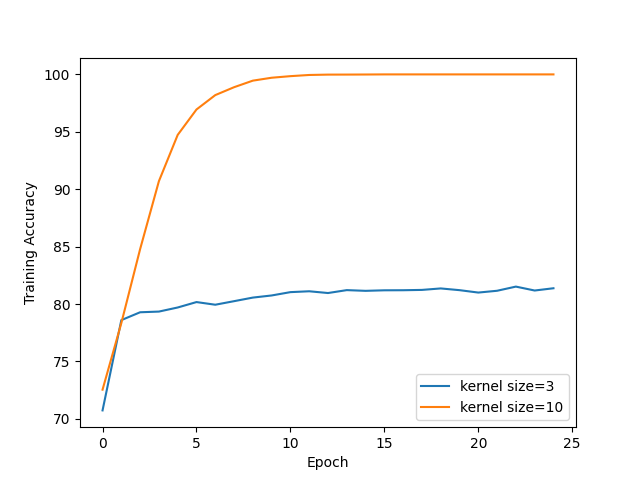
\includegraphics[scale=0.65]{c3vc10.png}\\
  \item[(d)]
  \item[(e)]
\end{enumerate}



 


\end{enumerate}
\end{document}
